\section{Results}
\label{sec:results}

\subsection{Where the limit lies}
\label{sec:res-limit}

\textbf{Selection objective (E0).} Selecting hyperparameters under the pinball loss instead of RMSE lowers mean pinball loss from 0.02545 to 0.02529 ($-0.66\%$) and MAE from 0.0682 to 0.0673 ($-1.4\%$), and raises skill from 0.4311 to 0.4351. The gain sits where theory puts it: pinball loss falls 1.4\% at P50 and 0.45\% at P90 and rises 0.1\% at P25. Squared error targets the conditional mean, so the preliminary configuration suited the tails least. The skill gain, +0.0040, is about 60\% of what the ensemble feature adds (+0.0065; Section~\ref{sec:res-widening}).

\textbf{Fleet oracle (E1).} Adding the contemporaneous output of every other rooftop raises $R^2$ from 0.7998 to 0.8226 and skill from 0.4194 to 0.4535 (Fig.~\ref{fig:ceiling}a). Perfect regional weather knowledge is therefore worth 0.0228 in $R^2$. With the oracle, geometry and metadata but no NWP, the model reaches $R^2$ 0.7076 and skill 0.2983. Knowing what the regional sky did recovers most of what the operational model achieves; NWP adds about 0.09 in $R^2$ beyond it. Regional-scale weather information is thus largely extracted already, and what remains unexplained is not regional.

\textbf{Residual structure (E2).} Residual autocorrelation is 0.715 at 15~min, 0.556 at 30~min, 0.407 at 1~h and 0.236 at 2~h, and falls to 0.015 at 24~h (Fig.~\ref{fig:ceiling}b). An error that is smooth over hours and uncorrelated from day to day is neither bias nor noise. It is the signature of a cloud field displaced in time or space. It also explains why persistence-based and day-to-day bias corrections fail here: yesterday's error says almost nothing about today's.

\begin{figure}[!htb]
\centering
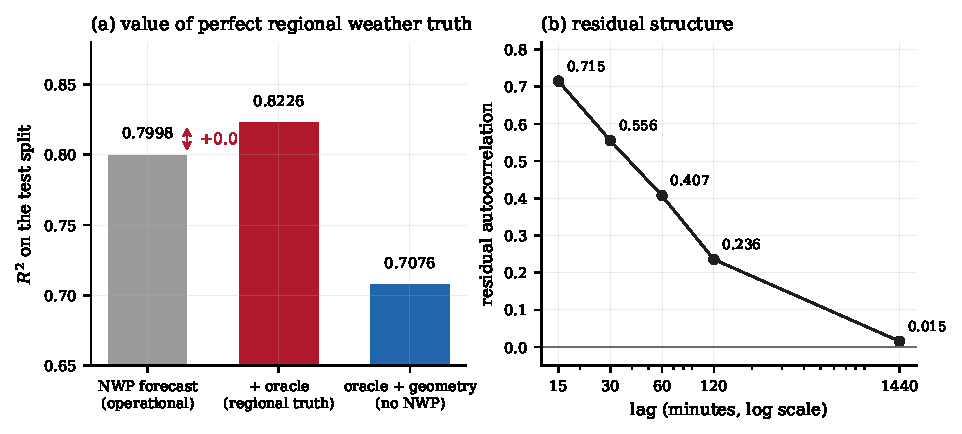
\includegraphics[width=\textwidth]{figures/fig4_ceiling.pdf}
\caption{(a) Test $R^2$ of the operational features, the same plus the fleet oracle, and the oracle without NWP. (b) Residual autocorrelation against lag.}
\label{fig:ceiling}
\end{figure}

\subsection{Where the error lives}
\label{sec:res-location}

Accuracy depends strongly on cloud (Fig.~\ref{fig:error}a). Binned by forecast clear-sky index, $R^2$ is 0.847 for clear slots ($n = 97{,}845$), but 0.440 in the 0.2--0.4 band and 0.480 in the 0.4--0.6 band. Overcast slots give 0.572 on a target standard deviation of only 0.063. Clear skies supply more than half the daylight slots and carry the pooled score; in broken cloud, where a storage controller most needs accuracy, the model explains under half the variance. Binning by the observed index reverses the sign of the conditional bias (overcast MBE +0.009 by forecast bins, $-0.068$ by observed bins), which matters when comparing with studies that condition on observed sky.

The irradiance forecast shows the same pattern against SARAH-3 (Fig.~\ref{fig:error}b). Absolute error is largest in partly cloudy conditions (RMSE 101.2~W\,m$^{-2}$) and smallest under overcast (54.9~W\,m$^{-2}$), but relative to available light the order reverses: nMAE is 36.8\% overcast, 32.4\% partly cloudy and 13.3\% clear.

The error belongs to the weather model, not to the rooftop (Fig.~\ref{fig:error}c). Across 31 rooftops spanning about $180 \times 210$~km, the ratio of the standard deviation to the median of irradiance RMSE is 0.033 in partly cloudy conditions, 0.029 in clear and 0.080 in overcast. An error driven by shading, orientation or microclimate would vary across two degrees of latitude. This one does not, so no per-rooftop feature or local calibration can remove it.

\begin{figure}[!htb]
\centering
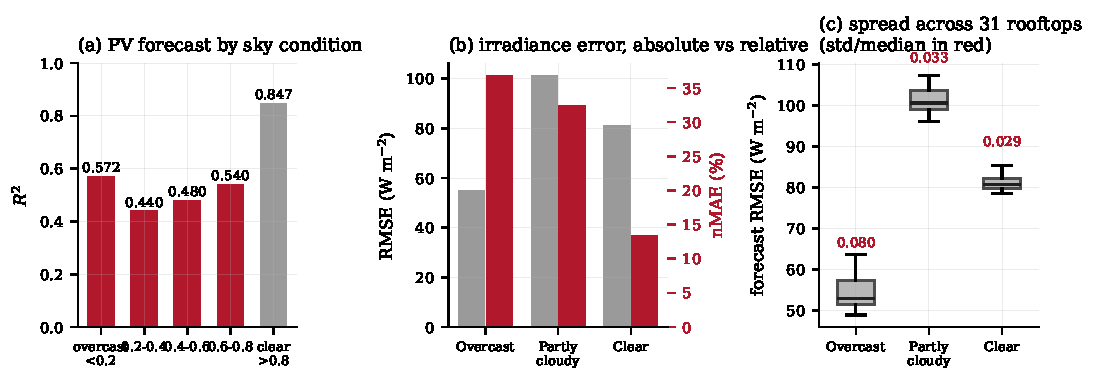
\includegraphics[width=\textwidth]{figures/fig5_error_location.pdf}
\caption{(a) PV forecast $R^2$ by forecast clear-sky index. (b) Irradiance forecast error against SARAH-3, absolute (RMSE) and relative (nMAE). (c) Per-rooftop irradiance RMSE across 31 systems.}
\label{fig:error}
\end{figure}

\subsection{Widening the weather input}
\label{sec:res-widening}

Table~\ref{tab:ablation} gives the ensemble ablation (E3). Only the multi-model mean improves every metric: skill rises from 0.4285 to 0.4351 and pinball loss falls from 0.02558 to 0.02529. Averaging ECMWF's own runs from one to three days before the target gives skill 0.4291, within noise of the baseline. Re-runs of one model are staler but not independent; centres differ in physics and therefore in error. Ensemble dispersion as a predictor lowers skill (0.4280), raises pinball loss by 1.6\% and lowers P25--P90 coverage from 0.622 to 0.592. The quantile model already infers conditional uncertainty from the clear-sky index and solar geometry, so dispersion adds mostly noise. All ten ensemble features together give a slightly higher $R^2$ but worse pinball loss and the lowest coverage (0.590).

\begin{table}[!htb]
\centering
\caption{Ensemble ablation on the chronological split, 32 systems.}
\label{tab:ablation}
\small
\begin{tabularx}{\textwidth}{@{}X c c c c@{}}
\toprule
Feature set & Features & $R^2$ & Skill & Pinball \\
\midrule
Base & 12 & 0.8070 & 0.4285 & 0.02558 \\
\textbf{+ multi-model mean (6 centres)} & 13 & \textbf{0.8114} & \textbf{0.4351} & \textbf{0.02529} \\
+ mean of all 12 members & 13 & 0.8078 & 0.4298 & 0.02552 \\
+ ensemble-mean POA & 13 & 0.8081 & 0.4301 & 0.02554 \\
+ lagged mean (ECMWF, days 1--3) & 13 & 0.8074 & 0.4291 & 0.02559 \\
+ ensemble spread only & 17 & 0.8066 & 0.4280 & 0.02598 \\
+ all 10 ensemble features & 22 & 0.8089 & 0.4314 & 0.02582 \\
\bottomrule
\end{tabularx}
\end{table}

\subsection{Proposed configuration and calibration}
\label{sec:res-config}

Table~\ref{tab:ablation} uses 32 systems because one rooftop was excluded (E4). With all 33 systems and no ensemble feature, $R^2$ is 0.7960 and skill 0.4139. Excluding system 81376 raises $R^2$ by 0.0110; adding the ensemble feature raises it by a further 0.0044, to 0.8114 (skill 0.4351). Two-thirds of the total gain comes from removing one rooftop. System 81376 holds 3.08\% of test rows but 7.69\% of squared error. Its defect is time-varying: in April--May 2026, inside the test window, its output relative to the fleet median fell to 0.60, against 0.85 and 0.89 in the same months of 2024 and 2025. This 31\% drop is the largest in the fleet (median $-3\%$), so no capacity value fixed during training can absorb it.
%% Source: v3_ensemble/src/eval/system_drift.py (season-matched April-May comparison).

Raw quantiles are over-confident at the upper tail: empirical coverage of the nominal P90 is 0.869 (Fig.~\ref{fig:recal}). Three offsets fitted on validation ($+0.0004$, $+0.0022$ and $+0.0105$ for P25, P50 and P90) bring coverage to 0.263, 0.520 and 0.912 against nominal 0.25, 0.50 and 0.90. Mean pinball loss is unchanged (0.02529 to 0.02527), and P25--P90 coverage moves from 0.614 to 0.649 against the nominal 0.65. The small over-coverage at P90 reflects validation-to-test drift and errs on the safe side for storage scheduling.

\begin{figure}[!htb]
\centering
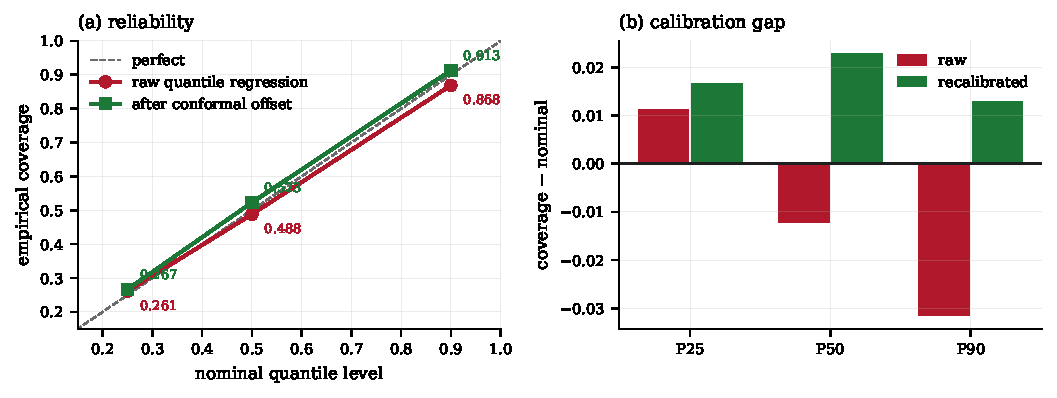
\includegraphics[width=\textwidth]{figures/fig7_recalibration.pdf}
\caption{Reliability of the proposed configuration before and after recalibration. (a) Empirical against nominal coverage. (b) Calibration gap per quantile.}
\label{fig:recal}
\end{figure}

\subsection{Irradiance correction and the reference}
\label{sec:res-mos}

\textbf{Reference.} Over the study window, the same ECMWF forecast scored against ERA5 has RMSE 51.1~W\,m$^{-2}$ and bias $-1.5$~W\,m$^{-2}$; against SARAH-3 it has 86.6~W\,m$^{-2}$ and $+9.2$~W\,m$^{-2}$. ERA5 understates RMSE by a factor of 1.69 (relative RMSE 16.5\% against 29.0\%) and reverses the sign of the bias. An external check supports the satellite figure: its bias is close to the +8~W\,m$^{-2}$ that \citet{Tuononen2019} measured for ECMWF IFS with ground instruments over four years at a comparable latitude.
%% Source: v3_ensemble/src/eval/reference_comparison.py (253,419 hourly rows, 31 systems; RMSE 86.63 vs 51.14, rRMSE 28.99 vs 16.52).

\textbf{Irradiance stage.} Against SARAH-3, random forest lowers MAE from 55.49 to 51.96~W\,m$^{-2}$ ($-6.4\%$) and RMSE from 86.27 to 81.94~W\,m$^{-2}$, raising $R^2$ from 0.866 to 0.879. Ridge regression barely changes MAE ($-0.5\%$) but cuts the bias from +11.40 to +0.88~W\,m$^{-2}$, which shows the bias is systematic. LightGBM and XGBoost make MAE worse ($-0.6\%$ and $-1.9\%$). Against ERA5, every learner degrades the forecast (MAE $-1.0\%$ to $-9.6\%$), because the raw bias against ERA5 is only +0.81~W\,m$^{-2}$ and there is nothing to learn. Trained against a reanalysis from the same model, MOS appears ineffective for the wrong reason.

\textbf{Power stage, seen rooftops.} The out-of-fold correction lowers test MAE from 55.49 to 52.13~W\,m$^{-2}$ ($-6.1\%$) and bias from +11.40 to +3.12~W\,m$^{-2}$ ($-73\%$). In the PV model it changes $R^2$ from 0.8114 to 0.8111 and skill from 0.4351 to 0.4346, and raises pinball loss from 0.02529 to 0.02539. Adding the correction as two extra features instead is slightly worse (0.8109, 0.4344, 0.02549).

\textbf{Power stage, unseen rooftops.} On a rooftop absent from training, the model cannot have absorbed that rooftop's share of the bias, so MOS should matter more. It does not. Across 33 held-out rooftops the median change is +0.00012 in $R^2$ and +0.00016 in skill; 17 of 33 rooftops improve, and changes range from $-0.0166$ to $+0.0361$. The largest gains are on 94362 (+0.0361) and 81376 (+0.0196), two of the worst-transferring rooftops, where the irradiance correction partly offsets a capacity error (Section~\ref{sec:res-deploy}); neither becomes usable. After 30 days of capacity + bias calibration, median skill is 0.3281 with MOS and 0.3230 without.

The reason is proportion. MOS removes about 8~W\,m$^{-2}$ of systematic bias, but RMSE falls only from 86.3 to 82.2~W\,m$^{-2}$. The remainder is the displacement error of Section~\ref{sec:res-limit}, which no statistical bias correction can reach, and the PV model has already fitted around the systematic part.

\subsection{Deployment on an unseen rooftop}
\label{sec:res-deploy}

A rooftop absent from training receives median $R^2$ 0.704 and skill 0.347, against 0.811 and 0.435 pooled over known rooftops on the chronological split. The tail matters more than the median: mean $R^2$ is 0.658, the 10th percentile 0.497 and the worst $-0.158$. Two of 33 rooftops, about one in sixteen, score worse than persistence.

\textbf{Hyperparameters for transfer.} Table~\ref{tab:transfer} and Fig.~\ref{fig:deploy} compare three configurations on the same 33 rooftops. The configuration that wins on the chronological split is the worst on unseen rooftops: mean $R^2$ 0.588, worst case $-0.985$, five failures. Selecting against held-out systems leaves the median almost unchanged but raises the 10th percentile from 0.308 to 0.496, lifts the worst rooftop to $-0.156$ and halves the failures. The transfer configuration has depth 4 and L2 penalty 4.34, against depth 15 and 0.008 for the temporal one. A depth-4 tree cannot encode rooftop identity and must learn what rooftops share.
%% Table 4 comes from tune_transfer.py (fixed seed); the E5 values above from consolidate.py (default seed). Same configuration; the 0.005 difference in median R2 is bagging-seed variation.

\begin{table}[!htb]
\centering
\caption{Zero-shot $R^2$ and skill on 33 held-out rooftops for three hyperparameter configurations. Failures: skill $\le 0$.}
\label{tab:transfer}
\small
\begin{tabularx}{\textwidth}{@{}X c c c c c c@{}}
\toprule
Configuration & Median & Mean & P10 & Worst & Median skill & Failures \\
\midrule
Preliminary (RMSE, temporal) & 0.719 & 0.603 & 0.378 & $-0.709$ & 0.293 & 4 \\
Tuned on temporal split & 0.708 & 0.588 & 0.308 & $-0.985$ & 0.316 & 5 \\
\textbf{Tuned on held-out systems} & 0.710 & \textbf{0.657} & \textbf{0.496} & $\mathbf{-0.156}$ & \textbf{0.340} & \textbf{2} \\
\bottomrule
\end{tabularx}
\end{table}

\begin{figure}[!htb]
\centering
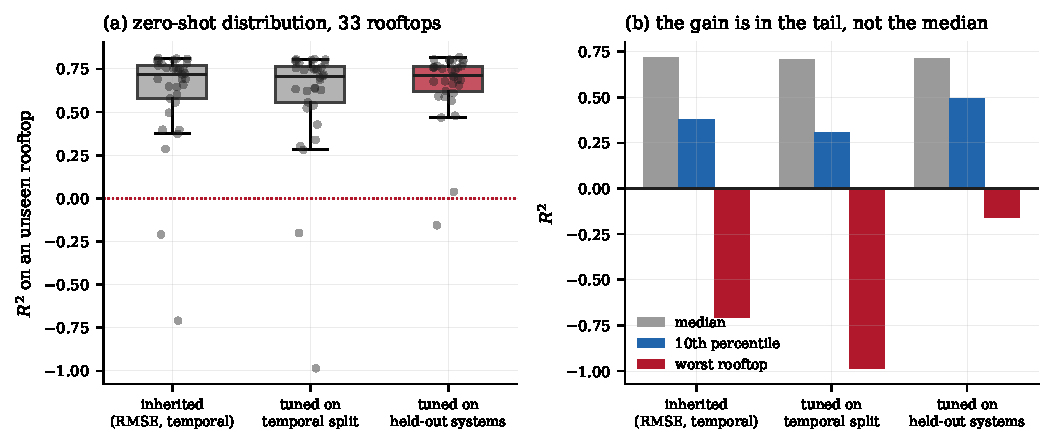
\includegraphics[width=\textwidth]{figures/fig8_deployment.pdf}
\caption{Zero-shot $R^2$ on 33 held-out rooftops for three configurations. (a) Distributions with individual rooftops. (b) Median, 10th percentile and worst case.}
\label{fig:deploy}
\end{figure}

\textbf{Rated capacity.} On unseen rooftops, the capacity ratio $P_{99}/C_\mathrm{p}$ (Section~\ref{sec:data-meta}) correlates with forecast bias at +0.709. The model learns the fleet-average relation between output and nameplate. A rooftop whose nameplate overstates its real capacity is over-forecast, and one whose nameplate understates it is under-forecast. On the chronological split this is hidden, because the model memorises each rooftop's scale. The lowest ratio in the fleet, 0.568, belongs to 94362 ($R^2$ 0.067); the worst rooftop, 81376 ($R^2$ $-0.158$), has a ratio of 0.693, also in the lowest fifth.

\textbf{Local calibration (E5).} Fig.~\ref{fig:calib} shows median skill against the length of the local window. Below about 30 days every correction is harmful: at 3 days, linear rescaling gives skill $-0.110$ against 0.347 uncorrected, because two parameters are fitted to a window that may contain no clear day. From 30 days, correction helps and linear rescaling is best, by +0.009 skill at 30 days, +0.022 at 45 and +0.053 at 60. Median $R^2$ rises from 0.704 at day 0 to 0.755 with linear rescaling at 45 days. The operating rule is no correction before 30 days of local history, then linear rescaling on a rolling window.

\begin{figure}[!htb]
\centering
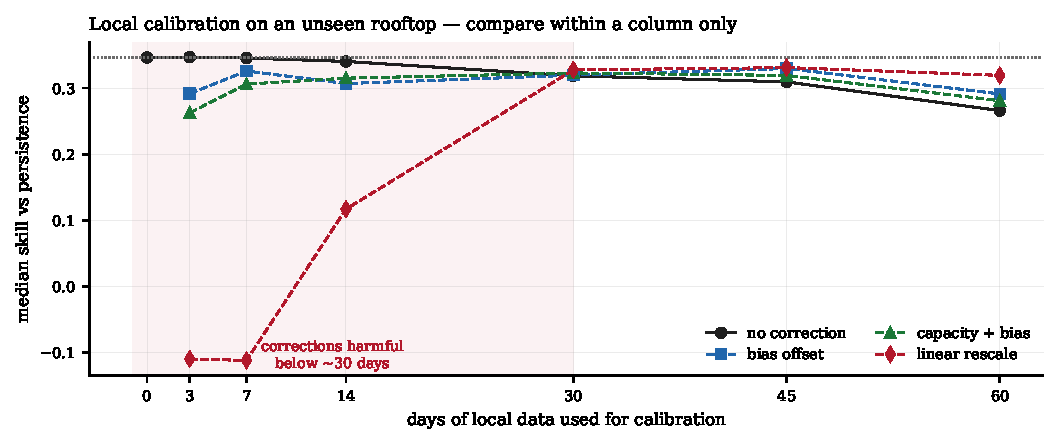
\includegraphics[width=\textwidth]{figures/fig9_calibration_sweep.pdf}
\caption{Median skill on held-out rooftops against local calibration window, by correction method. The shaded region marks where correction is harmful. Compare methods only at the same window length.}
\label{fig:calib}
\end{figure}

\subsection{Comparison with published results}
\label{sec:res-compare}

Cross-study comparison is unreliable. Accuracy depends on climate, horizon, resolution, aggregation and plant type, and on conventions: the same forecast here has normalised RMSE of 11.0\% of capacity but 38.0\% of mean output. Skill depends on the reference \citep{Yang2019}. \citet{Visser2019}, for example, report skill against smart persistence, a stronger reference than the plain persistence used here, so the two skills are not comparable. Utility-scale probabilistic results such as \citet{MayerYang2023} use a different normaliser and score. The comparisons that do hold are qualitative: tree ensembles were also the best learners on 152 distributed systems \citep{Visser2019}; input outweighs model family at day-ahead \citep{Nguyen2026}; and the 30-day calibration threshold has the same order of magnitude as the two months a local model needs in \citet{Depoortere2025}. The bias check in Section~\ref{sec:res-mos} supports the measurement chain. We do not claim higher accuracy than published work: Section~\ref{sec:res-limit} shows the accuracy of any learner here is bounded by the input.
